\section{Bases de datos NoSQL: Grafos (Neo4j)}

Neo4J viene ya instalado en la máquina virtual que estamos usando, por lo que simplemente debemos arrancar el servicio con el comando \texttt{sudo systemctl start neo4j}. Trabajaremos desde la interfaz \textit{web} en \texttt{http://localhost:7474}. Esta nos da celdas para introducir consultas en Cypher, el lenguaje de Neo4J, y proporciona una visualización gráfica de los resultados (si lo permiten) y en forma de tablas. \\

\subsection{Creación de índices}

Lo primero es crear la estructura de nodos y enlaces adecuada para las consultas. Iremos describiendola poco a poco, pero antes introduciremos los índices necesarios para que las consultas pensadas sean eficientes:

\begin{minted}[frame=single, fontsize=\footnotesize]{cypher}
CREATE INDEX IF NOT EXISTS FOR (j:Jugador) ON (j.id);
CREATE INDEX IF NOT EXISTS FOR (et:EdicionTorneo) ON (et.torneo, et.fecha);
CREATE INDEX IF NOT EXISTS FOR (p:Partido) ON (p.num_partido, p.fecha);
CREATE INDEX IF NOT EXISTS FOR (p:Pais) ON (p.codigo_iso2);
CREATE INDEX IF NOT EXISTS FOR (t:Torneo) ON (t.id);
\end{minted}

La indexación de las originales claves primarias en las tablas de relacionales resulta en consultas mucho más eficientes. Esto lo hacemos para \texttt{Jugador}, \texttt{EdicionTorneo}, \texttt{Pais} y \texttt{Torneo}. Para facilitar la búsqueda de partidos específicos, se indexan simplemente el número de partido y la fecha.

\subsection{Carga de datos con JBDC}

Al estar los datos almacenados dentro de un SGBDs relacional, usaremos JDBC para acceder directamente gestor y recuperar los datos. A continuación, creamos vamos creando la base de datos de grafos a la vez que cargamos los datos de la base de datos relacional. iremos describiendo poco a poco los nodos y relaciones que compondrán la nueva BD. Comenzamos creamos nodos para los paises, con sus correspondientes atributos de la tabla relacional. 

\begin{minted}[frame=single, fontsize=\footnotesize]{cypher}
WITH "jdbc:postgresql://localhost:5432/tenis?user=alumnogreibd&password=greibd2021" as url
CALL apoc.load.jdbc(url, "SELECT codigo_iso2, codigo_iso3, codigo_ioc, nombre FROM pais") YIELD row
CREATE (p:Pais {
codigo_iso2: row.codigo_iso2,
codigo_iso3: row.codigo_iso3,
codigo_ioc: row.codigo_ioc,
nombre: row.nombre
});
\end{minted}


Creamos nodos para los jugadores, con sus correspondientes atributos de la tabla relacional. Se crea una relación \texttt{REPRESENTA\_A} entre el nodo del país y el nodo del jugador, para indicar que el jugador representa a su país. Para ello, se usa \texttt{MATCH} para encontrar el nodo del país correspondiente al jugador, se crea el nodo del jugador y, posteriormente, se crea la relación (saliente desde el nodo jugador hacia el nodo país).

\begin{minted}[frame=single, fontsize=\footnotesize]{cypher}
WITH "jdbc:postgresql://localhost:5432/tenis?user=alumnogreibd&password=greibd2021" AS url
CALL apoc.load.jdbc(url, 
    "SELECT id, nombre, apellido, diestro, fecha_nacimiento, pais, altura FROM jugador") YIELD row
MATCH (pa:Pais {codigo_iso2: row.pais})
CREATE (j:Jugador {
    id: row.id,
    nombre: row.nombre,
    apellido: row.apellido,
    diestro: row.diestro,
    fecha_nacimiento: row.fecha_nacimiento,
    altura: row.altura
})
CREATE (j)-[:REPRESENTA_A]->(pa);
\end{minted}

Nodos para los torneos, con sus correspondientes atributos de la tabla relacional. Se crea una relación \texttt{SE\_CELEBRA\_EN} entre el nodo del país y el nodo del torneo, para indicar que el torneo se celebra en un país. Para ello, se usa \texttt{MATCH} para encontrar el nodo del país correspondiente al torneo, se crea el nodo del torneo y, posteriormente, se crea la relación (saliente desde el nodo torneo hacia el nodo país).

\begin{minted}[frame=single, fontsize=\footnotesize]{cypher}
// cargamos los torneos
WITH "jdbc:postgresql://localhost:5432/tenis?user=alumnogreibd&password=greibd2021" AS url
CALL apoc.load.jdbc(url, "SELECT id, nombre, pais FROM torneo") YIELD row
CREATE (t:Torneo {
    id: row.id,
    nombre: row.nombre
})
WITH t, row
OPTIONAL MATCH (pa:Pais {codigo_iso2: row.pais})
WITH t, pa
WHERE pa IS NOT NULL
CREATE (t)-[:SE_CELEBRA_EN]->(pa);
\end{minted}

Nodos para las ediciones de los torneos, con sus correspondientes atributos de la tabla relacional. Se crea una relación \texttt{EDICION\_DE} entre el nodo de la edición del torneo y el nodo del torneo, para indicar que la edición del torneo pertenece a un cierto torneo. Para ello, se usa \texttt{MATCH} para encontrar el nodo del torneo correspondiente a la edición del torneo, se crea el nodo de la edición del torneo y, posteriormente, se crea la relación (saliente desde el nodo edición del torneo hacia el nodo torneo).

\begin{minted}[frame=single, fontsize=\footnotesize]{cypher}
// cargamos las ediciones de los torneos
WITH "jdbc:postgresql://localhost:5432/tenis?user=alumnogreibd&password=greibd2021" AS url
CALL apoc.load.jdbc(url, "SELECT torneo, fecha, superficie, tamano, nivel FROM edicion_torneo") YIELD row
MATCH (t:Torneo {id: row.torneo})
CREATE (et:EdicionTorneo {
    fecha: row.fecha,
    superficie: row.superficie,
    tamano: row.tamano,
    nivel: row.nivel,
    torneo: row.torneo
})
CREATE (et)-[:EDICION_DE]->(t);
\end{minted}

A continuación, cargamos los partidos creando nodos con sus correspondientes atributos de la tabla relacional. Esta creación dio varios problemas debido al conflicto con el \textit{left join} que comentamos en la sección de agregados; con una carga estándar se omitían partidos, y por tanto la consulta 4 no devolvía los resultados esperados. Para solucionar esto, se ha optado por crear primero el nodo del partido y, posteriormente, se crean las relaciones con los jugadores, torneos y ganadores/perdedores. La creación de las mismas la haremos con un \texttt{OPTIONAL MATCH} para que se cree la relación si existe el nodo al que se quiere enlazar, pero en caso negativo, se incluya el resto de datos del partido igualmente. Además, se ha añadido un \texttt{LIMIT} para evitar problemas de rendimiento: la carga se hizo de 10000 en 10000, cambiando el \texttt{OFFSET} en cada carga. \\

\noindent Vamos un poco más en detalle con las relaciones:
\begin{itemize}
\item \texttt{SE\_JUEGA\_EN}: Relación desde el nodo del partido hacia el nodo del torneo, para indicar que el partido se juega en un cierto torneo. Esta relación se crea con un \texttt{OPTIONAL MATCH} para que se cree la relación si existe el nodo del torneo al que se quiere enlazar, pero en caso negativo, se incluya el resto de datos del partido igualmente.
\item \texttt{GANADO\_POR}: Relación desde el nodo del partido hacia el nodo del jugador, para indicar que el partido ha sido ganado por un cierto jugador. Esta relación se crea con un \texttt{OPTIONAL MATCH} para que se cree la relación si existe el nodo del jugador al que se quiere enlazar, pero en caso negativo, se incluya el resto de datos del partido igualmente. Además, esta relación contiene como atributos las estadísticas del ganador en ese partido. 
\item \texttt{PERDIDO\_POR}: Relación completamente análoga a la anterior, pero para el perdedor del partido.
\end{itemize}

\begin{minted}[frame=single, fontsize=\footnotesize]{cypher}
// cargamos los partidos
WITH "jdbc:postgresql://localhost:5432/tenis?user=alumnogreibd&password=greibd2021" AS url
CALL apoc.load.jdbc(url,
"SELECT * FROM partido p LIMIT 10000 OFFSET 0") YIELD row

CREATE (p:Partido {
num_partido: row.num_partido,
fecha: row.fecha,
num_sets: row.num_sets,
ronda: row.ronda,
desenlace: row.desenlace,
torneo_id: row.torneo 
})

// vinculamos con el torneo si existe
WITH p, row
OPTIONAL MATCH (t:Torneo {id: row.torneo})
WITH p, row, t
WHERE t IS NOT NULL
CREATE (p)-[:SE_JUEGA_EN]->(t)

// vinculamos con el ganador si existe
WITH p, row
OPTIONAL MATCH (ganador:Jugador {id: toInteger(row.ganador)})
WITH p, row, ganador
WHERE ganador IS NOT NULL
CREATE (p)-[:GANADO_POR {
num_aces: row.num_aces_ganador,
num_dob_faltas: row.num_dob_faltas_ganador,
num_ptos_servidos: row.num_ptos_servidos_ganador,
num_primeros_servicios: row.num_primeros_servicios_ganador,
num_primeros_servicios_ganados: row.num_primeros_servicios_ganados_ganador,
num_segundos_servicios_ganados: row.num_segundos_servicios_ganados_ganador,
num_juegos_servidos: row.num_juegos_servidos_ganador,
num_break_salvados: row.num_break_salvados_ganador,
num_break_afrontados: row.num_break_afrontados_ganador
}]->(ganador)

// vinculamos con el perdedor si existe
WITH p, row
OPTIONAL MATCH (perdedor:Jugador {id: toInteger(row.perdedor)})
WITH p, row, perdedor
WHERE perdedor IS NOT NULL
CREATE (p)-[:PERDIDO_POR {
num_aces: row.num_aces_perdedor,
num_dob_faltas: row.num_dob_faltas_perdedor,
num_ptos_servidos: row.num_ptos_servidos_perdedor,
num_primeros_servicios: row.num_primeros_servicios_perdedor,
num_primeros_servicios_ganados: row.num_primeros_servicios_ganados_perdedor,
num_segundos_servicios_ganados: row.num_segundos_servicios_ganados_perdedor,
num_juegos_servidos: row.num_juegos_servidos_perdedor,
num_break_salvados: row.num_break_salvados_perdedor,
num_break_afrontados: row.num_break_afrontados_perdedor
}]->(perdedor);
\end{minted}

Por último, cargamos los sets de los partidos con los atributos de la tabla relacional homónima. Se crea una relación \texttt{PERTENECE\_A} desde el nodo del set del partido hacia el nodo del partido, para indicar que el set pertenece a un cierto partido. Para ello, se usa \texttt{OPTIONAL MATCH} para encontrar el nodo del partido correspondiente al set del partido, y, si se encuentra, crea el nodo del set del partido y, posteriormente, se crea la relación. La carga de estos datos también la haremos de 10000 en 10000 para evitar problemas de rendimiento.

\begin{minted}[frame=single, fontsize=\footnotesize]{cypher}
// cargamos los sets de los partidos
WITH "jdbc:postgresql://localhost:5432/tenis?user=alumnogreibd&password=greibd2021" AS url
CALL apoc.load.jdbc(url,
"SELECT * FROM sets_partido LIMIT 10000 OFFSET 0") YIELD row
OPTIONAL MATCH (p:Partido {num_partido: row.num_partido, fecha: row.fecha})
WITH row, p
WHERE p IS NOT NULL
CREATE (sp:SetPartido {
num_set: row.num_set,
juegos_ganador: row.juegos_ganador,
juegos_perdedor: row.juegos_perdedor,
puntos_tiebreak_perdedor: row.puntos_tiebreak_perdedor
})
CREATE (sp)-[:PERTENECE_A]->(p);
\end{minted}


\subsection{Consultas}

Con la base de datos de grafos ya creada, podemos realizar las mismas consultas que llevamos realizando durante todo el documento. Para aligerar la cantidad de texto en las explicaciones posteriores, vamos a comentar algunos detalles de la sintáxis del código, comunes a todas las consultas, de modo que en la descripción de cada consulta podamos dar un enfoque menos técnico (al conocer ya de antemano esos detalles) y más semántico. 
\begin{itemize}
\item Para indicar una relación entre dos nodos, usamos \texttt{-->}. Con el signo $->$ indicamos la dirección de la relación, es decir, con $->$ indicacom que la relación va desde el nodo de la izquierda hacia el de la derecha, y con $<-$ indicamos que la relación va desde el nodo de la derecha hacia el de la izquierda.
\item La relación entre ambos nodos la especificaremos entre corchetes, como por ejemplo \texttt{-[:RELACION]->}, y podemos agregar un alias en caso de que queramos referirnos a la relación, por ejemplo \texttt{-[r:RELACION]->}. En caso de ser una relación con atributos, podemos añadirlos entre llaves, como por ejemplo \texttt{-[:RELACION \{atributo1: valor1, atributo2: valor2\}]->}.
\item Los nodos los especificamos entre paréntesis, por ejemplo \texttt{()}. Si queremos hacer referencia a ello, podemos añadir un alias, por ejemplo \texttt{(n)}. En caso de querer referirnos a un tipo de nodo concreto, añadimos el tipo, por ejemplo \texttt{(n:TipoNodo)}.
\item La estructura básica de las consultas comenzará con un \texttt{MATCH} para buscar patrones en el grafo, seguirá con un \texttt{WHERE} para filtrar los resultados (como haciamos en SQL), y finalmente un \texttt{RETURN} para mostrar los resultados. En varias consultas queremos hacer cálculos sobre los resultados; para ello usamos \texttt{WITH}, que nos permite pasar los resultados de una cláusula a otra. Al igual que en SQL, podemos usar \texttt{ORDER BY} para ordenar los resultados.
\end{itemize}

Con todo esto, si queremos, por ejemplo, buscar patrones de partidos ganados por un jugador en cierto torneo, usaremos un patrón de búsqueda en el \texttt{MATCH} de tipo 
\begin{equation*}
    \texttt{(j:Jugador)<-[:GANADO\_POR]-(p:Partido)-[:SE\_JUEGA\_EN]->(t:Torneo)}
\end{equation*}

Usamos las relaciones ya creadas, un partido es ganado por un jugador (relación desde el partido hacia el jugador) y se juega en un torneo (relación desde el partido hacia el torneo). Especificamos un alias para cada nodo e indicamos el tipo de nodo entre los paréntesis. \\

Tras esta breve introducción de los detalles sintácticos más básicos de este lenguaje, mostramos las consultas en Cypher que hemos realizado en Neo4J para obtener los mismos resultados que en las consultas SQL. \\

\subsubsection{Muestra todos los ganadores del torneo ``Wimbledon'' (Nombre apellidos y año). Ordena el resultado por año.}

Para esta consulta, curiosamente, nos sirve el ejemplo que pusimos antes. Queremos buscar jugadores que hayan ganado el partido de la ronda final de un torneo concreto, Wimbledon. Para esto, partimos de nodos tipo \texttt{Partido} y buscamos los nodos de tipo \texttt{Jugador} y de tipo \texttt{Torneo} que se relacionen con ese partido mediante las relaciones \texttt{GANADO\_POR} y \texttt{SE\_JUEGA\_EN}, respectivamente. Al buscar esta patrón, debemos filtrar o seleccionar solo los nodos de partidos que correspondan a rondas finales, y el nodo de torneo Wimbledon; esto lo hacemos con el \texttt{where}, como en SQL. \\

Con el \texttt{RETURN} mostramos el nombre y apellido de los jugadores que cumplen con el patrón, así como el año de la edición del torneo en el que ganaron. Para obtener el año, convertimos la fecha a string, con \texttt{toString()}, y nos quedamos con los 4 primeros caracteres de esa cadena de texto, que son el año; esto lo conseguimos con \texttt{substring}, fijando como caracter inicial el 0 y final el 3 (4 no incluido). Finalmente, ordenamos el resultado de forma ascendente con el \texttt{ORDER BY ano}. \\

\begin{minted}[frame=single, fontsize=\footnotesize]{cypher}
MATCH (j:Jugador)<-[gp:GANADO_POR]-(p:Partido)-[:SE_JUEGA_EN]->(t:Torneo)
WHERE t.nombre = 'Wimbledon'
AND p.ronda = 'F'
RETURN j.nombre AS nombre,
j.apellido AS apellido,
substring(toString(p.fecha), 0, 4) AS ano
ORDER BY ano;
\end{minted}

\begin{figure}[H]
\centering
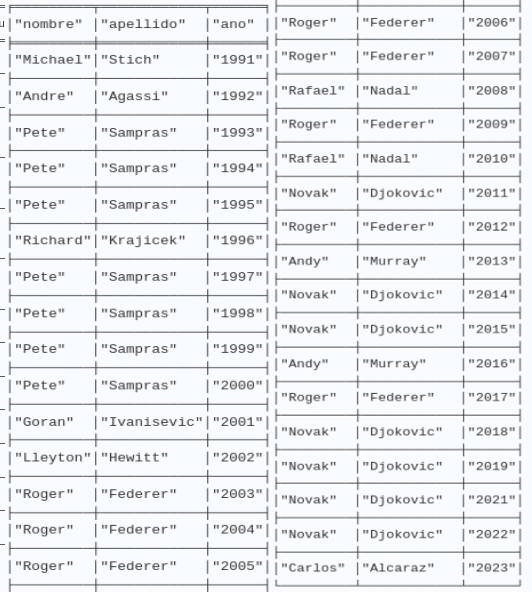
\includegraphics[width=0.35\textwidth]{fotos/q1_neo.png}
\caption{Modelo de grafos en Neo4J, consulta 1. Al no caber la visualización de la tabla completa en la pantalla, se recortó la imagen por la mitad y se compone en dos partes para mostrar la tabla completa.}
\label{fig:q1_neo}
\end{figure}



\subsubsection{Muestra los años en los que Roger Federer ganó algún torneo de nivel Gran Slam (G) o Master 1000 (M). Para cada año, muestra el número de torneos y lista sus nombres (ordenados por la fecha de celebración). Ordena el resultado por el año}



\begin{minted}[frame=single, fontsize=\footnotesize]{cypher}
MATCH (j:Jugador)<-[:GANADO_POR]-(p:Partido)-[:SE_JUEGA_EN]->(t:Torneo)
MATCH (et:EdicionTorneo)-[:EDICION_DE]->(t)
WHERE j.nombre = 'Roger'
AND j.apellido = 'Federer'
AND p.ronda = 'F'
AND et.nivel IN ['G', 'M']
AND et.fecha = p.fecha
AND et.torneo = t.id
WITH substring(toString(p.fecha), 0, 4) AS ano, 
     collect({nombre: t.nombre, fecha: p.fecha}) AS torneos
UNWIND torneos AS torneo
WITH ano, torneo.nombre AS nombre, torneo.fecha AS fecha
ORDER BY fecha
RETURN ano, count(DISTINCT nombre) AS num_torneos, 
    reduce(s = head(collect(nombre)), x IN tail(collect(nombre)) | s + ', ' + x) AS torneos
ORDER BY ano;
\end{minted}

\begin{figure}[H]
\centering
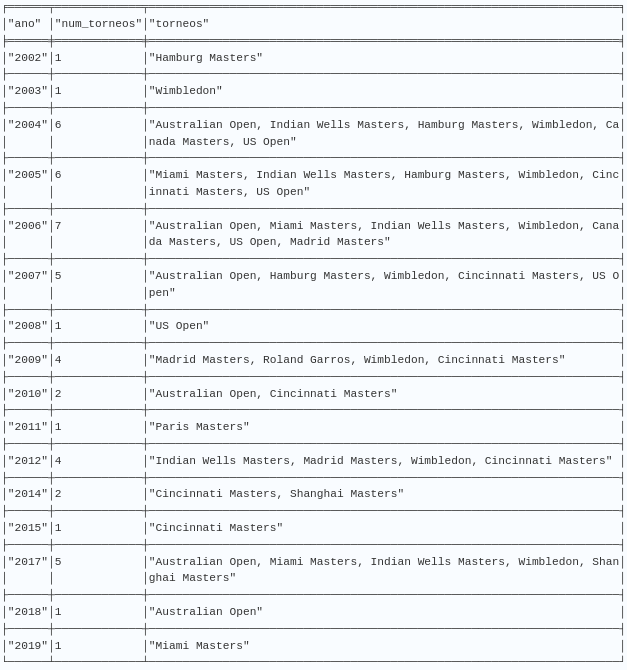
\includegraphics[width=0.45\textwidth]{fotos/q2_neo.png}
\caption{Modelo de grafos en Neo4J, consulta 2.}
\label{fig:q2_neo}
\end{figure}



\subsubsection{Muestra los partidos de semifinales (ronda='SF') y final (ronda = 'F') del torneo de "Roland Garros" del 2018. Para cada partido muestra la ronda, el tipo de desenlace, el nombre y apellidos del ganador y el nombre y apellidos del perdedor y el resultado con el número de juegos del ganador y del perdedor en cada set, y opcionalmente en paréntesis el número de juegos del perdedor en el tie break}

\begin{minted}[frame=single, fontsize=\footnotesize]{cypher}
MATCH (jg:Jugador)<-[:GANADO_POR]-(p:Partido)-[:PERDIDO_POR]-(jp:Jugador),
(p)-[:SE_JUEGA_EN]->(t:Torneo),
(sp:SetPartido)-[:PERTENECE_A]->(p)
WHERE t.nombre = 'Roland Garros'
AND p.ronda IN ['SF', 'F']
AND substring(toString(p.fecha), 0, 4) = '2018'
WITH p, jg, jp, sp
ORDER BY sp.num_set
WITH p, jg, jp,
collect(sp.juegos_ganador + '-' + sp.juegos_perdedor +
CASE sp.puntos_tiebreak_perdedor
WHEN null THEN ''
ELSE '(' + toString(sp.puntos_tiebreak_perdedor) + ')'
END) as sets
RETURN p.ronda as ronda,
p.desenlace as desenlace,
jg.nombre + ' ' + jg.apellido as ganador,
jp.nombre + ' ' + jp.apellido as perdedor,
reduce(s = head(sets), x IN tail(sets) | s + ', ' + x) as resultado
ORDER BY p.fecha;
\end{minted}

\begin{figure}[H]
\centering
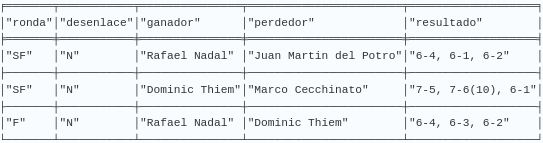
\includegraphics[width=0.65\textwidth]{fotos/q3_neo.png}
\caption{Modelo de grafos en Neo4J, consulta 3.}
\label{fig:q3_neo}
\end{figure}





\subsubsection{Muestra la lista de jugadores españoles (ES) que ganaron algún torneo de nivel Gran Slam (G). Para cada jugador muestra los siguientes datos resumen de todos sus partidos: número de partidos jugados, porcentaje de victorias, porcentaje de aces, porcentaje de dobles faltas, porcentaje de servicios ganados, porcentaje de restos ganados, porcentaje de break points salvados (de los sufridos en contra), porcentaje de break points ganados (de los provocados a favor)}

\begin{minted}[frame=single, fontsize=\footnotesize]{cypher}
// buscamos jugadores españoles que han ganado finales de Grand Slam (para eliminar duplicados, sino lo haciamos directamente con las estadísticas)
MATCH (j:Jugador)-[:REPRESENTA_A]->(p:Pais {codigo_iso2: 'ES'})
MATCH (j)<-[:GANADO_POR]-(partido:Partido)-[:SE_JUEGA_EN]->(t:Torneo)
MATCH (et:EdicionTorneo)-[:EDICION_DE]->(t)
WHERE partido.ronda = 'F'
AND et.nivel = 'G'
AND et.fecha = partido.fecha
AND et.torneo = t.id
WITH DISTINCT j.id AS id_jugador, j.nombre + ' ' + j.apellido AS jugador

// calculamos las estadísticas de estos jugadores
MATCH (j:Jugador)
WHERE j.id = id_jugador
MATCH (p:Partido)
MATCH (j)<-[r:GANADO_POR|PERDIDO_POR]-(p)
// necesitamos las estadisticas de sus rivales
OPTIONAL MATCH (p)-[rp:PERDIDO_POR]->(rival_j:Jugador)
OPTIONAL MATCH (p)-[rg:GANADO_POR]->(rival_g:Jugador)
WITH jugador, p, j, r, type(r) AS tipo, rp, rg,
CASE type(r) WHEN 'GANADO_POR' THEN 1 ELSE 0 END AS es_ganador,
r.num_aces AS aces,
r.num_ptos_servidos AS ptos_servidos,
r.num_dob_faltas AS dobles_faltas,
r.num_primeros_servicios_ganados + r.num_segundos_servicios_ganados AS servicios_ganados,
// restos ganados
CASE type(r)
WHEN 'GANADO_POR' THEN rp.num_ptos_servidos - rp.num_primeros_servicios_ganados - rp.num_segundos_servicios_ganados
ELSE rg.num_ptos_servidos - rg.num_primeros_servicios_ganados - rg.num_segundos_servicios_ganados END AS restos_ganados,
CASE type(r)
WHEN 'GANADO_POR' THEN rp.num_ptos_servidos
ELSE rg.num_ptos_servidos END AS ptos_servidos_rival,
r.num_break_salvados AS breaks_salvados,
r.num_break_afrontados AS breaks_afrontados,
CASE type(r)
WHEN 'GANADO_POR' THEN rp.num_break_afrontados - rp.num_break_salvados
ELSE rg.num_break_afrontados - rg.num_break_salvados END AS breaks_ganados,
CASE type(r)
WHEN 'GANADO_POR' THEN rp.num_break_afrontados
ELSE rg.num_break_afrontados END AS breaks_rival

WITH jugador,
count(p) AS partidos,
100.0 * sum(es_ganador) / count(p) AS pcje_victorias,
CASE WHEN sum(ptos_servidos) = 0 THEN 0
ELSE 100.0 * sum(aces) / sum(ptos_servidos) END AS pcje_aces,
CASE WHEN sum(ptos_servidos) = 0 THEN 0
ELSE 100.0 * sum(dobles_faltas) / sum(ptos_servidos) END AS pcje_dobles_faltas,
CASE WHEN sum(ptos_servidos) = 0 THEN 0
ELSE 100.0 * sum(servicios_ganados) / sum(ptos_servidos) END AS pcje_servicios_ganados,
CASE WHEN sum(ptos_servidos_rival) = 0 THEN 0
ELSE 100.0 * sum(restos_ganados) / sum(ptos_servidos_rival) END AS pcje_restos_ganados,
CASE WHEN sum(breaks_afrontados) = 0 THEN 0
ELSE 100.0 * sum(breaks_salvados) / sum(breaks_afrontados) END AS pcje_breaks_salvados,
CASE WHEN sum(breaks_rival) = 0 THEN 0
ELSE 100.0 * sum(breaks_ganados) / sum(breaks_rival) END AS pcje_breaks_ganados
RETURN
jugador,
partidos,
round(pcje_victorias, 1) AS pcje_victorias,
round(pcje_aces, 1) AS pcje_aces,
round(pcje_dobles_faltas, 1) AS pcje_dobles_faltas,
round(pcje_servicios_ganados, 1) AS pcje_servicios_ganados,
round(pcje_restos_ganados, 1) AS pcje_restos_ganados,
round(pcje_breaks_salvados, 1) AS pcje_breaks_salvados,
round(pcje_breaks_ganados, 1) AS pcje_breaks_ganados
ORDER BY jugador;
\end{minted}

\begin{figure}[H]
\centering
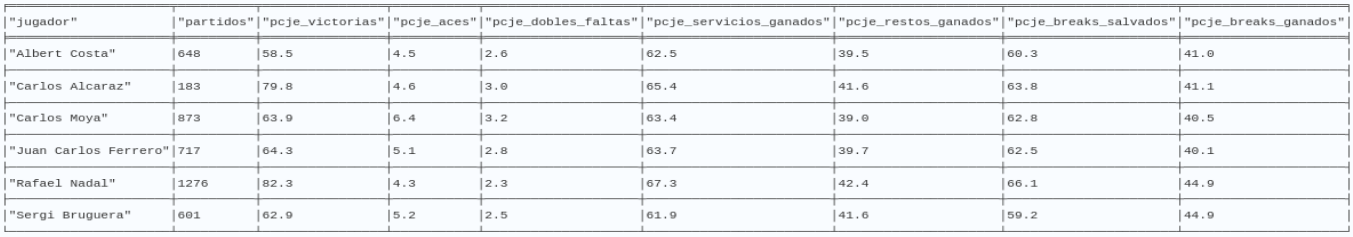
\includegraphics[width=\textwidth]{fotos/q4_neo.png}
\caption{Modelo de grafos en Neo4J, consulta 4.}
\label{fig:q4_neo}
\end{figure}





\subsubsection{Lista los jugadores que fueron derrotados (en algún partido del 2018) por el rival de Rafael Nadal de la primera ronda (R128) de Roland Garros de 2018}

\begin{minted}[frame=single, fontsize=\footnotesize]{cypher}
// encontramos al rival de Nadal en Roland Garros 2018 R128
MATCH (nadal:Jugador {nombre: 'Rafael', apellido: 'Nadal'})
MATCH (rival:Jugador)
MATCH (p:Partido)-[:SE_JUEGA_EN]->(t:Torneo {nombre: 'Roland Garros'})
WHERE p.ronda = 'R128'
AND substring(toString(p.fecha), 0, 4) = '2018'
AND ((nadal)<-[:GANADO_POR]-(p)-[:PERDIDO_POR]->(rival) OR
(nadal)<-[:PERDIDO_POR]-(p)-[:GANADO_POR]->(rival))


// buscamos los partidos donde este rival perdió en 2018
WITH rival
MATCH (rival)<-[:GANADO_POR]-(derrotas:Partido)-[:PERDIDO_POR]->(perdedor:Jugador)
WHERE substring(toString(derrotas.fecha), 0, 4) = '2018'
MATCH (perdedor)-[:REPRESENTA_A]->(pais:Pais)
RETURN DISTINCT
perdedor.nombre + ' ' + perdedor.apellido as jugador,
pais.codigo_iso2 as pais
ORDER BY jugador;
\end{minted}

\begin{figure}[H]
\centering
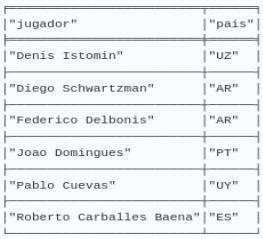
\includegraphics[width=0.25\textwidth]{fotos/q5_neo.png}
\caption{Modelo de grafos en Neo4J, consulta 5.}
\label{fig:q5_neo}
\end{figure}